\section*{Math 202A - HW10 - Dan Davison - \texttt{ddavison@berkeley.edu}}

\begin{mdframed}
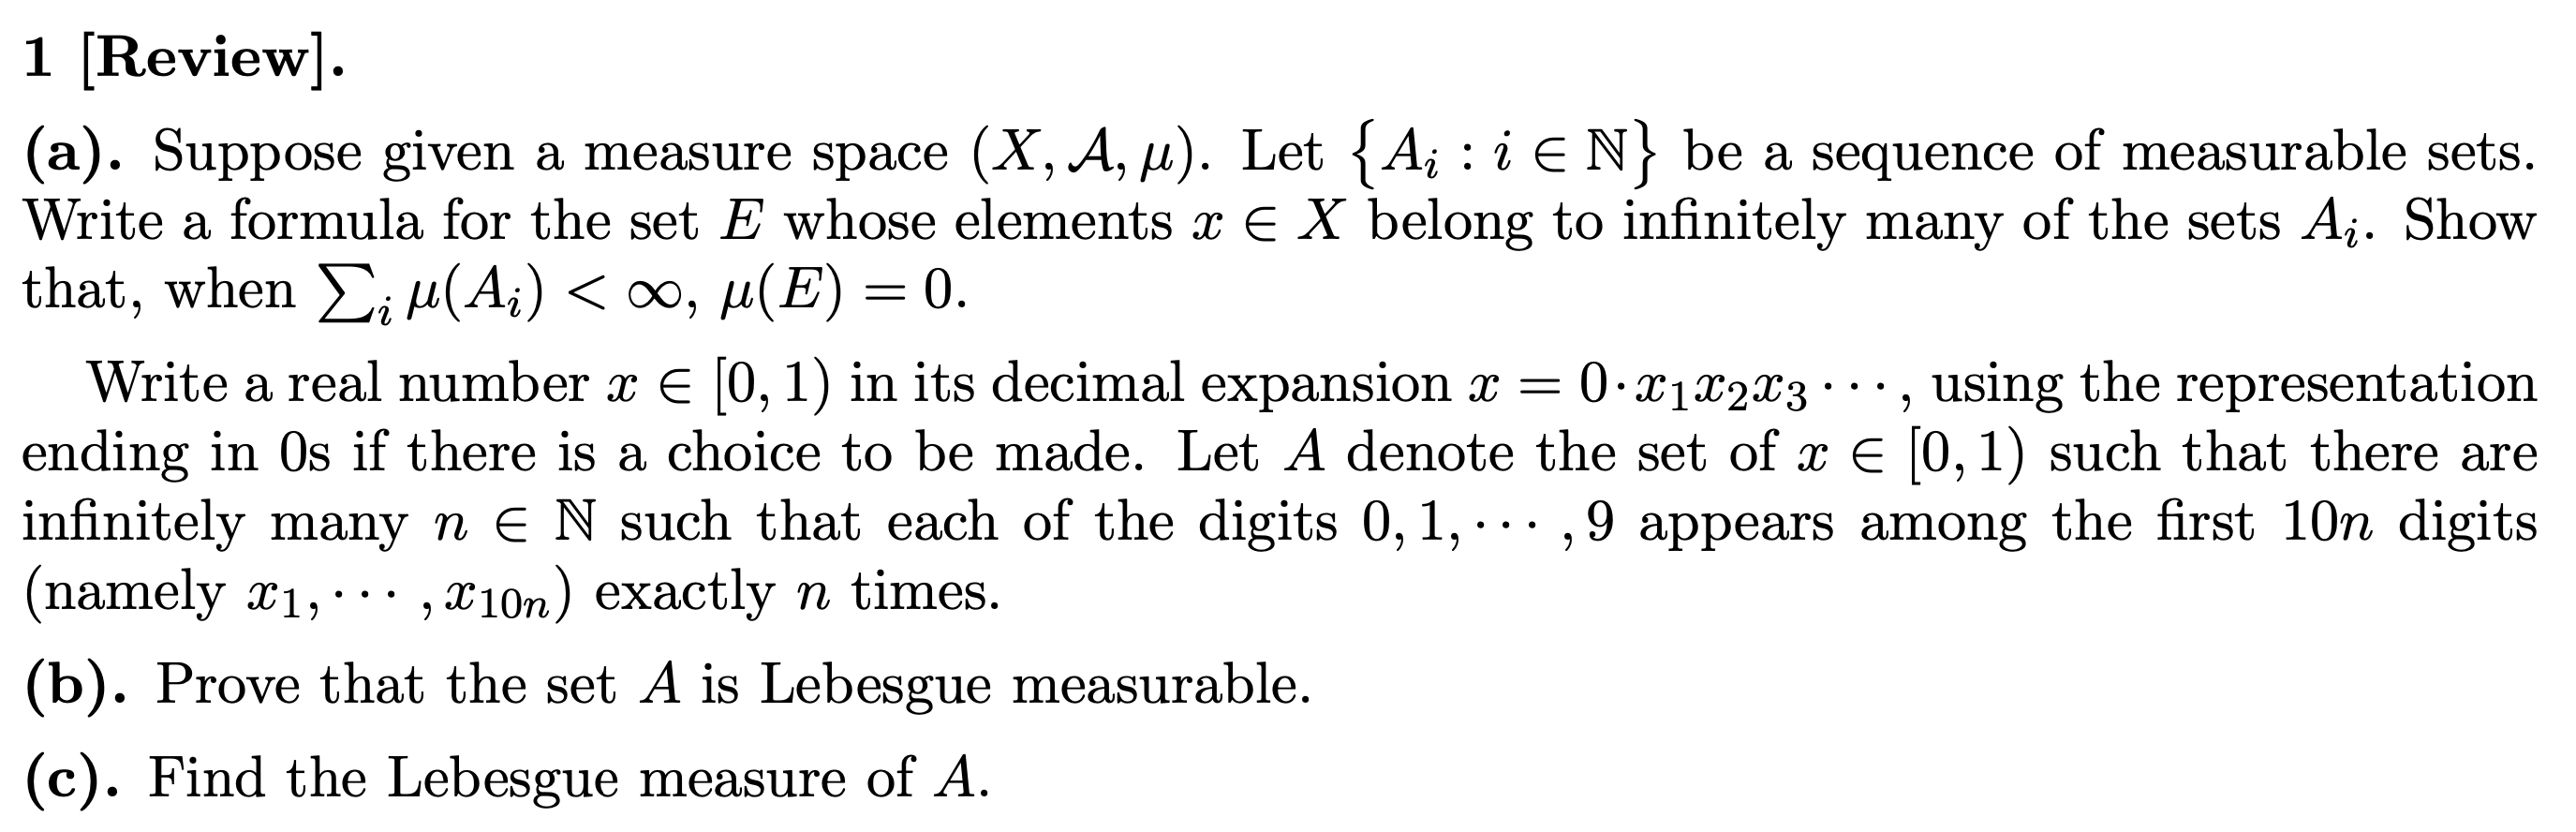
\includegraphics[width=400pt]{img/analysis--berkeley-202a-hw10-7127.png}
\end{mdframed}

\begin{enumerate}[label=(\alph*)]

\item ~\\
  \begin{align*}
    E = \bigcup_{n \in \ms{N}} \bigcap_{i=1}^\infty A_{n_i}
  \end{align*}

  $E = \bigcap_{i=1}^\infty A_i$ is a set whose elements belong to infinitely many of the sets $A_i$. (There are others, for example $\bigcap_{i=2}^\infty A_i$.)

  \begin{claim*}
    If $\sum_i \mu(A_i) < \infty$ then $\mu\(\bigcap_{i=1}^\infty A_i\) = 0$.
  \end{claim*}

  \begin{proof}
    First note that $\inf \{\mu(A_i) ~:~ i \in \N\} = 0$. To see this, suppose for a contradiction
    that $\inf \{\mu(A_i) ~:~ i \in \N\} = a > 0$; but then $\sum_i \mu(A_i) \geq \sum_i a = \infty$.

    Let $\eps > 0$. Then, since $\inf \{\mu(A_i) ~:~ i \in \N\} = 0$, there exists $i$ such that $\mu(A_i) < \eps$.

    Next note that $\(\bigcap_{i=1}^\infty A_i\) \subseteq A_i$ for all $i \in \N$. Therefore by monotonicity
    of measure we have $\mu\(\bigcap_{i=1}^\infty A_i\) \leq \mu(A_i)$ for all $i \in \N$.

    Therefore we have $\mu\(\bigcap_{i=1}^\infty A_i\) \leq \eps$. But $\eps > 0$ is arbitrary,
    therefore $\mu\(\bigcap_{i=1}^\infty A_i\) = 0$.
  \end{proof}

\item ~\\

\end{enumerate}


\newpage
\begin{mdframed}
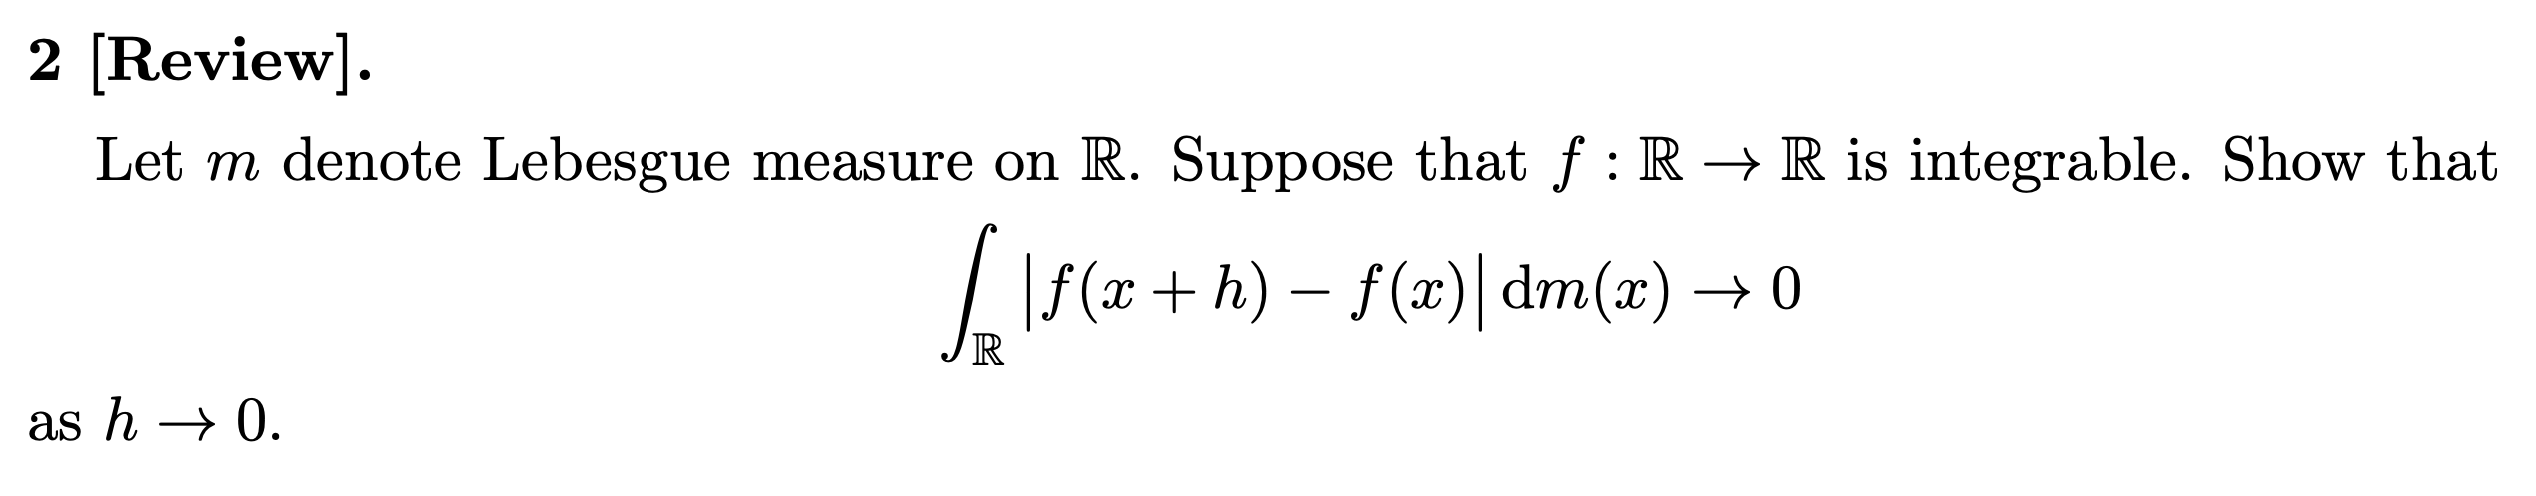
\includegraphics[width=400pt]{img/analysis--berkeley-202a-hw10-5e9e.png}
\end{mdframed}


\newpage
\begin{mdframed}
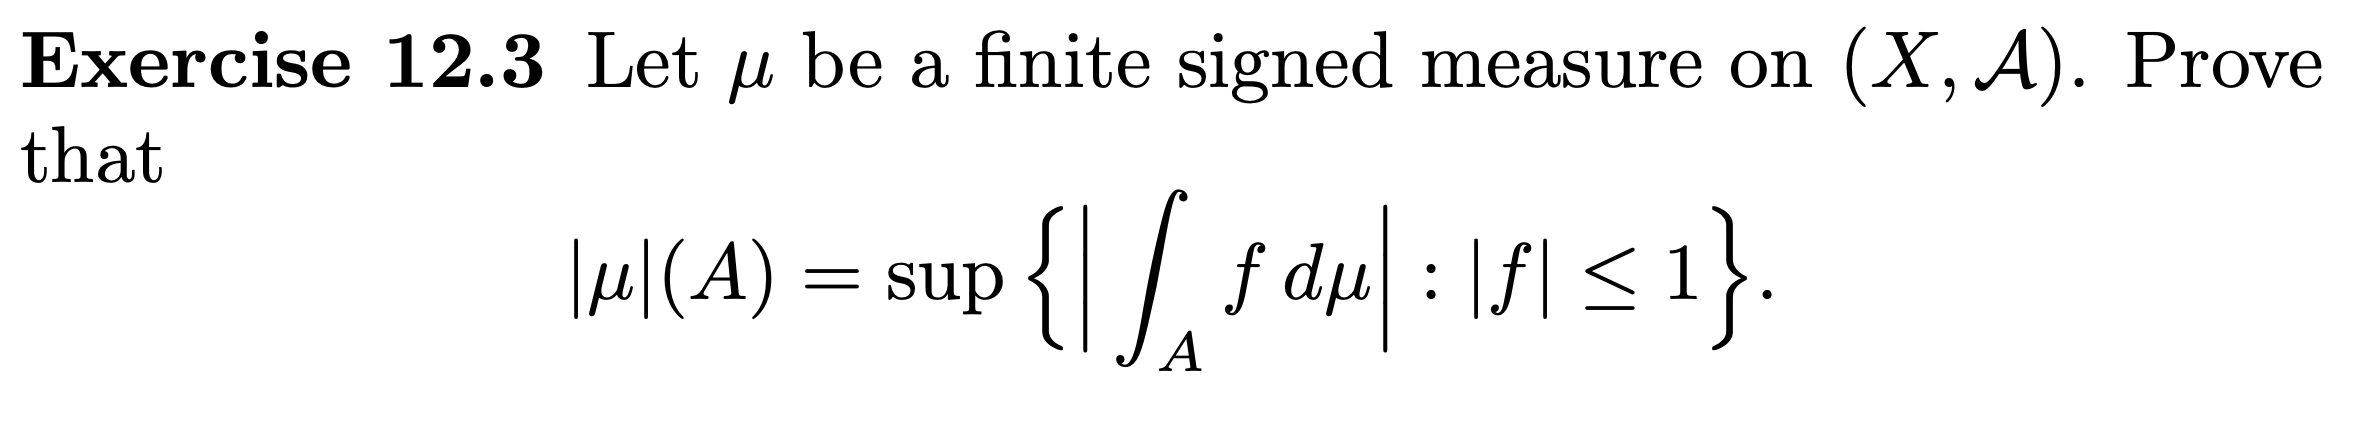
\includegraphics[width=400pt]{img/analysis--berkeley-202a-hw10-551e.png}
\end{mdframed}


\newpage
\begin{mdframed}
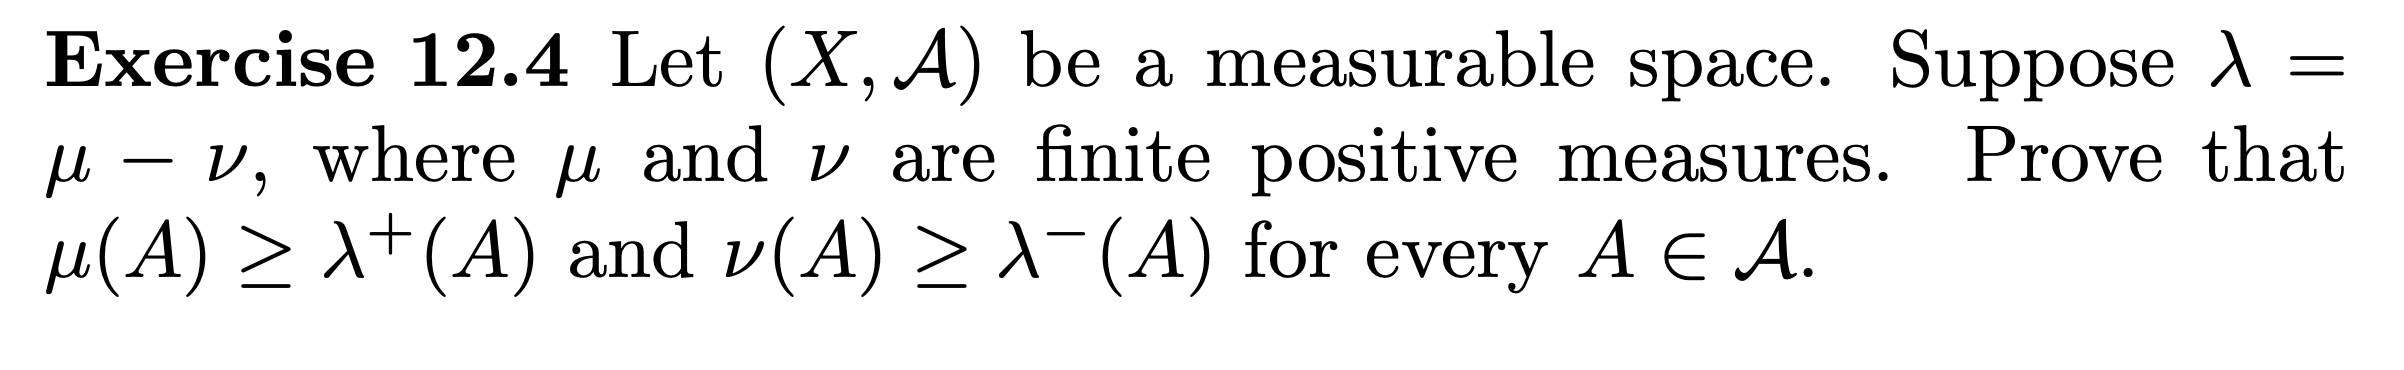
\includegraphics[width=400pt]{img/analysis--berkeley-202a-hw10-8336.png}
\end{mdframed}

\newpage
\begin{mdframed}
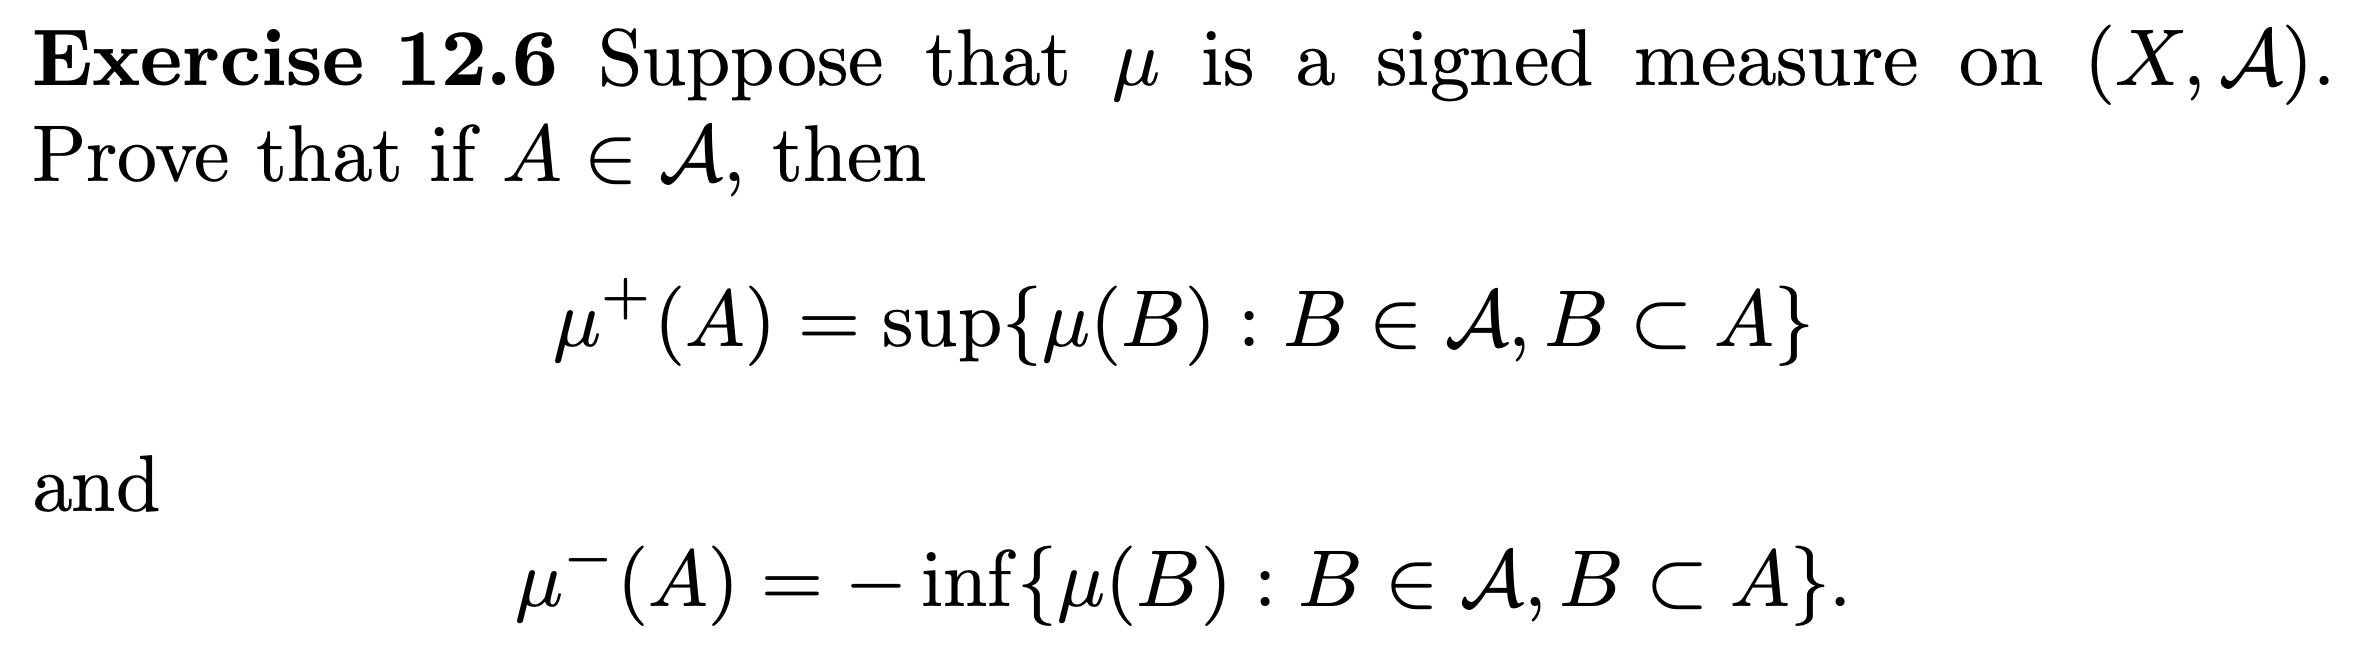
\includegraphics[width=400pt]{img/analysis--berkeley-202a-hw10-0220.png}
\end{mdframed}
